\documentclass{article}
% For math environments
\usepackage{amsmath, amsfonts}
% For links
\usepackage[colorlinks=true,
    linkcolor = blue,
    urlcolor  = blue,
    citecolor = blue,
    anchorcolor = blue]{hyperref}
% Put space between paragraphs
\usepackage{parskip}
% For figures
\usepackage{tikz}
% Set the margins to not be ridiculous
\usepackage[margin=0.75in]{geometry}
% For multiple columns
\usepackage{multicol}
% For controlling enum/itemize spacing and indentation
\usepackage{enumitem}
% More math symbols
\usepackage{amssymb}
% To change enumerate labels

% For tikz plots
\usepackage{pgfplots}
% This isn't needed but avoids a compiler warning
\pgfplotsset{compat=1.16}

% Allow multi-line equations to be broken across pages
\allowdisplaybreaks

% Use @ as a letter
\makeatletter

% Scale down all tikz coordinates while maintaining font size
\tikzset{every picture/.style={scale=0.45, every picture/.style={}}}


% Macros
% Monospace code
\def\code#1{\texttt{#1}}

% Greek letters
\def\a{\alpha}
\def\b{\beta}
\def\g{\gamma}
\def\d{\delta}
\def\D{\Delta}

% Commands that make life easier
\newcommand\gath[1]{\begin{gather} #1 \end{gather}}
\newcommand\ali[1]{\begin{align} #1 \end{align}}
\newcommand\parens[1]{\left( #1 \right)}
\newcommand\squares[1]{\left[ #1 \right]}
\newcommand\braces[1]{\left\{ #1 \right\}}
\newcommand\angles[1]{\left\langle #1 \right\rangle}
\newcommand\deriv[2]{\frac{d #1}{d #2}}
\newcommand\abs[1]{\left| #1 \right|}
\newcommand\floor[1]{\left\lfloor #1 \right\rfloor}
\DeclareMathOperator{\lcm}{lcm}
\def\non{\nonumber \\}

% Multiline equation space
\def\mlesp{\hspace{1.2cm}}

% For grid diagrams
\newcommand\gridbox[3]{\draw (#1,#2) rectangle (#1+1,#2+1) node[pos=.5] {#3};}
\newcommand\gridboxh[3]{\draw[fill=red!20] (#1,#2) rectangle (#1+1,#2+1) node[pos=.5] {#3};}
\newcommand\gridboxb[3]{\draw[fill=black] (#1,#2) rectangle (#1+1,#2+1) node[pos=.5] {#3};}
\newcommand\gridsym[3]{\node at (#1+0.5,#2+0.5) {$#3$};}
\newcommand\gridblank[2]{\filldraw[draw=gray, color=gray] (#1,#2) rectangle (#1+1,#2+1);}
\newcommand\gridcirc[2]{\draw (#1 + 0.5,#2 + 0.5) circle (0.25);}
\newcommand\cwlab[3]{
  \def\dd{0.15}
  \draw (#1 + \dd - 0.03, #2 + 1 - \dd) node {\scriptsize #3};
}

\def\bbw{3.5}
\def\bbh{2}
\newcommand\bigbox[3]{\draw (#1*\bbw,#2*\bbh) rectangle (#1*\bbw+\bbw,#2*\bbh+\bbh) node[pos=.5] {#3};}
\newcommand\bbtextr[3]{\node[right] at (#1*\bbw,#2*\bbh+0.5*\bbh) {#3};}
\newcommand\bbtextb[3]{\node[align=center] at (#1*\bbw+0.5*\bbw,#2*\bbh+0.5*\bbh) {#3};}

% Box puzzle stock answer
\newcommand\boxans[1]{
  Logic was used to deduce the solution:

  #1

  This was verified using Python as well as shown to be unique with a brute force approach.
}

% Multiple numbers
\newcommand\mn[1]{$#1$'s}

% Commands for problems
\newcommand\problem[4]{
  \section*{#1}

  Question: #3
  
  Answer: #2
  
  Explanation: #4
}
\newcommand\aproblem[4]{\problem{Dec #1}{#2}{#3}{#4}}
\newcommand\cproblem[4]{\problem{Problem #1}{#2}{#3}{#4}}

\def\advent@xxiv@i{
  Eve writes down five different positive integers.
  The sum of her integers is $16$. What is the product of her integers?
}

\def\advent@xxiv@ii{
  $14$ is the smallest even number that cannot be obtained by rolling two $6$-sided dice and finding the product of the numbers rolled.

  What is the smallest even number that cannot be obtained by rolling one hundred $100$-sided dice and finding the product of the numbers rolled?
}

\def\advent@xxiv@iii{
  There are $5$ ways to write $5$ as the sum of positive odd numbers:
  \begin{itemize}
    \item $1 + 1 + 1 + 1 + 1$
    \item $1 + 1 + 3$
    \item $3 + 1 + 1$
    \item $1 + 3 + 1$
    \item $5$
  \end{itemize}

  How many ways are there to write $14$ as the sum of positive odd numbers?
}

\def\advent@xxiv@iv{
  The geometric mean of a set of $n$ numbers is computed by mulitplying all the numbers together, then taking the $n$th root.
  The factors of $9$ are $1$, $3$, and $9$.
  The geometric mean of these factors is
  \gath{
    \sqrt[3]{1 \times 3 \times 9} = \sqrt[3]{27} = 3
  }
  What is the smallest number where the geometric mean of its factors is $13$?
}

\def\advent@xxiv@v{
  The sum of $11$ consecutive integers is $2024$.
  What is the smallest of the $11$ integers?
}

\def\advent@xxiv@vi{Put the digits 1 to 9 (using each digit exactly once) in the boxes so that the sums are correct. The sums should be read left to right and top to bottom ignoring the usual order of operations. For example, 4+3×2 is 14, not 10. Today's number is the product of the numbers in the red boxes.
  The number $n$ has $55$ digits.
  All of its digits are $9$.
  What is the sum of the digits of $n^3$?
}

\def\advent@xxiv@vii{
  What is the obtuse angle in degrees between the minute and hour hands of a clock at 08:22?
}

\def\advent@xxiv@viii{
  It is possible to arrange $4$ points on a plane and draw non-intersecting lines between them to form $3$ non-overlapping triangles:

  \begin{center}
    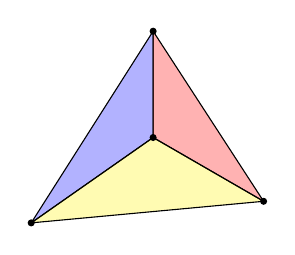
\begin{tikzpicture}
      \def\ds{3}
      \def\pa{(0: 0)}
      \def\pb{(90: \ds)}
      \def\pc{(215: 1.4*\ds)}
      \def\pd{(-30: 1.2*\ds)}

      \def\bcr{3}
      \def\scr{0.55*\bcr}
      \def\sca{34}
      \def\mcr{0.7*\bcr}
      \def\mca{142}
      \def\pr{0.1}

      % Triangles
      \draw[fill=blue,fill opacity=0.3] \pa -- \pb -- \pc -- cycle;
      \draw[fill=red,fill opacity=0.3] \pa -- \pb -- \pd -- cycle;
      \draw[fill=yellow,fill opacity=0.3] \pa -- \pd -- \pc -- cycle;

      % Points
      \fill \pa circle (\pr);
      \fill \pb circle (\pr);
      \fill \pc circle (\pr);
      \fill \pd circle (\pr);
    \end{tikzpicture}
  \end{center}

  It is not possible to make more than $3$ triangles with $4$ points.

  What is the maximum number of non-overlapping triangles that can be made by arranging $290$ points on a plane and drawing non-intersecting lines between them?
}

\def\advent@xxiv@ix{
  Put the digits $1$ to $9$ (using each digit exactly once) in the boxes so that the sums are correct.
  The sums should be read left to right and top to bottom ignoring the usual order of operations.
  For example, $4 + 3 \times 2$ is $14$, not $10$.
  Today's number is the product of the numbers in the red boxes.

  \grid@advent@xxiv@ix{}{}{}{}{}{}{}{}{}
}

\def\advent@xxiv@x{
  A number is a palindrome if it's the same when its digits are written in reverse order.

  What is the sum of all the numbers between $10$ and $100$ that are palindromes?
}

\def\advent@xxiv@xi{
  There are $6$ sets of integers between $1$ and $5$ (inclusive) that contain an odd number of numbers whose median value is $3$:

  \begin{itemize}
    \item $\braces{3}$
    \item $\braces{1,3,4}$
    \item $\braces{2,3,4}$
    \item $\braces{1,3,5}$
    \item $\braces{2,3,5}$
    \item $\braces{1,2,3,4,5}$
  \end{itemize}

  How many sets of integers between $1$ and $11$ (inclusive) are there that contain an odd number of numbers whose median value is $5$?
}

\def\advent@xxiv@xii{
  Holly picks a three-digit number.
  She then makes a two-digit number by removing one of the digits.
  The sum of her two numbers is $309$.
  What was Holly's original three-digit number?
}

\def\advent@xxiv@xiii{
  Today's number is given in this crossnumber.
  No number in the completed grid starts with $0$.

  \begin{multicols}{2}
    \crossnumstd{}{}{}{}{}{}{}{}{}

    \vfill\null
    \columnbreak

    \begin{center}
      \textbf{Across}

      \begin{tabular}{clc}
        \textbf{1} & Today's number.  & (\textbf{3}) \\
        \textbf{4} & Two times 5A.    & (\textbf{3}) \\
        \textbf{5} & A multiple of 1. & (\textbf{3})
      \end{tabular}

      \textbf{Down}

      \begin{tabular}{clc}
        \textbf{1} & Sum of digits is 15. & (\textbf{3}) \\
        \textbf{2} & Sum of digits is 19. & (\textbf{3}) \\
        \textbf{3} & Three times 5A.      & (\textbf{3})
      \end{tabular}
    \end{center}
  \end{multicols}
}

\def\advent@xxiv@xiv{
  $15^3$ is $3375$.
  The last $3$ digits of $15^3$ are $375$.

  What are the last $3$ digits of $15^{1234567890}$?
}

\def\advent@xxiv@xv{
  The number $2268$ is equal to the product of a square number (whose last digit is not $0$) and the same square number with its digits reversed: $36 \times 63$.

  What is the smallest three-digit number that is equal to the product of a square number (whose last digit is not $0$) and the same square number with its digits reversed?
}

\def\advent@xxiv@xvi{
  Put the digits $1$ to $9$ (using each digit exactly once) in the boxes so that the sums are correct.
  The sums should be read left to right and top to bottom ignoring the usual order of operations.
  For example, $4 + 3 \times 2$ is $14$, not $10$.
  Today's number is the product of the numbers in the red boxes.

  \grid@advent@xxiv@xvi{}{}{}{}{}{}{}{}{}
}

\def\advent@xxiv@xvii{
  The number $40$ has $8$ factors: $1$, $2$, $4$, $5$, $8$, $10$, $20$, and $40$.

  How many factors does the number $2^{26} \times 5 \times 7^5 \times 11^2$ have?
}

\def\advent@xxiv@xviii{
  TODO
}

\def\card@xxiv@i{
  What is the largest number you can make by using the digits $1$ to $4$ to make two $2$-digit numbers, then mutiplying the two numbers together?
}

\def\card@xxiv@ii{
  What is the largest number you can make by using the digits $0$ to $9$ to make a $2$-digit number and an $8$-digit number, then mutiplying the two numbers together?
}

\def\card@xxiv@iii{
  The expansion of $(2x+3)^2$ is $4x^2 + 12x + 9$.
  The sum of the coefficients of $4x^2 + 12x + 9$ is $25$.
  What is the sum of the coefficients of the expansion of $(30x + 5)^2$?
}

\def\card@xxiv@iv{
  What is the sum of the coefficients of the expansion of $(2x+1)^{11}$?
}

\def\card@xxiv@v{
  What is the geometric mean of all the factors of $41306329$?
}

\def\card@xxiv@vi{
  What is the largest number for which the geometric mean of all its factors is $92$?
}

\def\card@xxiv@vii{
  What is the sum of all the factors of $7^4$?
}

\def\card@xxiv@viii{
  How many numbers between $1$ and $28988500000$ have an odd number of factors?
}

\def\card@xxiv@ix{
  Eve found the total of the $365$ consecutive integers starting at $500$ and the total of the next $365$ consecutive integers, then subtracted the smaller total from the larger total.
  What was her result?
}

\def\card@xxiv@x{
  Eve found the total of the $n$ consecutive integers starting at a number and the total of the next $n$ consecutive integers, then subtracted the smaller total from the larger total.
  Her result was $22344529$.
  What is the largest possible value of $n$ that she could have used?
}


\begin{document}

\title{MS Scroggs Advent Calendar 2020 Answers}
\author{Dan Whitman}
\date{}

\maketitle

Answers: \href{https://www.mscroggs.co.uk/puzzles/advent2020}{https://www.mscroggs.co.uk/puzzles/advent2020}

\aproblem{1}{195}{\advent@xx@i}{
  The number of $r$-digit numbers formed using these digits is the number of permutations of the 5 digits, selecting $r$ of them.
  Hence the total number of numbers is the sum of these permutations from 1-digit numbers to 5-digit numbers:
  \gath{
    \sum_{r=1}^5 {}_5 P_r = \sum_{r=1}^5 \frac{5!}{(5-r)!} = 325 \,.
  }
  If interested only in the odd numbers, the least significant digit must be chosen from the 3 odd digits (1, 3, and 5) whereas the rest are chosen normally from the remaining digits.
  Thus the total number of odd numbers is reasoned to be
  \gath{
    \sum_{r=1}^5 \frac{3 \cdot 4!}{5 - r} = 195 \,.
  }

  This answer was also verified using a brute force Python program.
}

\aproblem{2}{124}{\advent@xx@ii}{
  For a square with sides of length $s$, the smallest circle in which the square can fit is reasoned to have a radius of $r = s / \sqrt{2}$.
  For a circle of radius $r$, the smallest square into which the circle can fit is reasoned to have sides of $s = 2r$.

  So, in our case, we have an initial square of area $a = 62$ and sides of $s = \sqrt{a}$.
  Hence the smallest circle containing this square has a radius of
  \gath{
    r = \frac{s}{\sqrt{2}} = \frac{\sqrt{a}}{\sqrt{2}} = \sqrt{\frac{a}{2}} \,.
  }
  The smallest square containing this circle then has sides of
  \gath{
    S = 2r = 2 \sqrt{\frac{a}{2}} = \sqrt{2a} \,.
  }
  Hence the area of this square is
  \gath{
    A = S^2 = 2a = 124 \,.
  }
}

\aproblem{3}{321}{\advent@xx@iii}{
  \boxans{\grid@advent@xx@iii{9}{1}{6}{4}{8}{2}{7}{3}{5}}
}

\aproblem{4}{371}{\advent@xx@iv}{
  Solved this using a brute force Python program.
}

\aproblem{5}{103}{\advent@xx@v}{
  For $n$ dice, the minimum possible sum is $n$ when they all roll a one.
  The maximum number is $6n$ when they all roll a six.
  Every sum $s$ such that $n \leq s \leq 6n$ is possible and occurs some number of times in the $6^n$ possible dice combinations.
  Obviously the sums $s = n$ and $s = 6n$ each occur only once.
  Let $N_n(s)$ be the number of combinations that sum $s$ occurs in the rolls of $n$ dice, which is of course directly related to the probability of that sum occurring.
  Though I was unable to prove it, some numerical experiments showed that all the values of $s$ are symmetric such that
  \gath{
    N_n(n + i) = N_n(6n - i)
  }
  for all integer $0 \leq i \leq 5n$.

  Letting $a = 200$ and $b = 521$, there must then be some integers $n$ and $i$ such that
  \ali{
    n + i &= a \non
    6n -i &= b
  }
  since these sums have the same probability.
  Thus this linear system can be solved:
  \gath{
    \begin{bmatrix}
      1 & 1 \\
      6 & -1
    \end{bmatrix}
    \begin{bmatrix}
      n \\ i
    \end{bmatrix}
    =
    \begin{bmatrix}
      a \\ b
    \end{bmatrix} \,.
  }
  Doing so results in $n = 103$ and $i = 97$, where of course $n$ is the number of dice and so is our answer.
}

\aproblem{6}{192}{\advent@xx@vi}{
  First, we notice that, if $N$ is the number of indistinguishable tokens used, then both the example and our actual problem are $2 \times 2N$ grids.
  We can use this to our advantage by considering only this special case.
  So first let $f(N)$ denote the number of valid placements of $N$ tokens on a $1 \times 2N$ grid.
  For a single token we have only a $1 \times 2$ grid, in which there are clearly only $f(1) = 2$ possible placements.
  Next consider a $1 \times 2N$ grid, where we divide the grid in to $N$ distinct $1 \times 2$ regions horizontally.
  Because we have $N$ tokens, it follows that the $n$th token is confined to the $n$th $1 \times 2$ region in order for all of the tokens to fit validly on the board.

  If the first token is positioned on the left side of its $1 \times 2$ grid as illustrated below,

  \newcommand\gridboxo[4]{\draw[fill=gray!20] (#1,#2) rectangle (#1+#3,#2+1) node[pos=.5] {#4};}
  \begin{center}
    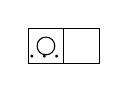
\begin{tikzpicture}
      \gridbox{0}{0}{}
      \gridcirc{0}{0}
      \gridbox{1}{0}{}
      \gridboxo{2}{0}{1}{}
      \gridboxo{3}{0}{2}{$\cdots$}
      \gridboxo{5}{0}{1}{}
    \end{tikzpicture}
  \end{center}
  
  then the remaining $N-1$ tokens can be placed freely on the remaining $1 \times 2(N-1)$ grid so that there are $f(N-1)$ of these placements.
  However, if the first token is on the right of its $1 \times 2$ grid, then this forces all of the remaining tokens to the right side of their $1 \times 2$ grids in order for the board to be valid

  \begin{center}
    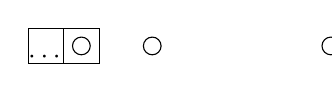
\begin{tikzpicture}
      \gridbox{0}{0}{}
      \gridbox{1}{0}{}
      \gridcirc{1}{0}
      \gridboxo{2}{0}{1}{}
      \gridboxo{3}{0}{1}{}
      \gridcirc{3}{0}
      \gridboxo{4}{0}{2}{$\cdots$}
      \gridboxo{6}{0}{1}{}
      \gridboxo{7}{0}{1}{}
      \gridcirc{7}{0}
    \end{tikzpicture}
  \end{center}
  
  and so clearly there is only one valid placement for this case.
  Thus the number of configurations for $N$ tokens is simply $f(N) = f(N-1) + 1$.
  So $f$ is defined by the following recursive relationship:
  \ali{
    f(1) &= 2 \non
    f(N) &= f(N-1) + 1 \,.
  }
  We can easily prove that $f(N) = N + 1$ by induction.
  First, clearly $f(1) = 1 + 1 = 2$ as required.
  Now suppose that $f(N) = N + 1$ so that
  \gath{
    f(N+1) = f((N+1) - 1) + 1 = f(N) + 1 = (N + 1) + 1 \,,
  }
  which shows the induction step.

  Now, one property that a general $2 \times m$ grid has is that, whether a token is on the upper or lower row, it blocks exactly the same spaces.
  Because of this, for a given valid placement on a $1 \times 2N$ grid with $N$ tokens, there are exactly $2^N$ valid placements on a $2 \times 2N$ grid, one for every combination where the tokens can either be on the upper or lower row.
  Think of binary numbers where a token on the lower row is a 0 and a token on the upper row is a 1.
  Thus the total number of valid placements for a $2 \times 2N$ grid with $N$ tokens is
  \gath{
    g(N) = 2^N f(N) = 2^N (N + 1) \,.
  }
  So, for the given example, we have $g(2) = 12$ as expected, and for the actual problem our answer is $g(5) = 192$.

  This answer was also verified using a brute force Python program.
}

\aproblem{7}{315}{\advent@xx@vii}{
  First, in general for non-negative integers $b \geq a$, we have
  \gath{
    \sum_{i=a}^b i = \sum_{i=0}^b i - \sum_{i=0}^{a-1} i = \frac{b(b+1)}{2} - \frac{a(a-1)}{2} = \frac{1}{2} [b(b+1) - a(a-1)] \,,
  }
  noting that this is valid even when $a = 0$ since this causes the second term to vanish.
  We also have
  \gath{
    \sum_{i=a}^b i^2 = \sum_{i=0}^b i^2 - \sum_{i=0}^{a-1} i^2 = \frac{b(b+1)(2b+1)}{6} - \frac{a(a-1)(2a-1)}{6} = \frac{1}{6} [b(b+1)(2b+1) - a(a-1)(2a - 1)] \,,
  }
  which is also valid when $a = 0$ for the same reason.

  Now consider the general case of all the dominoes with integers running from $a$ to $b$ (inclusive) so that of course $b \geq a$.
  Then the number of such dominoes is reasoned to be
  \ali{
    N(a, b) &= \sum_{i=a}^b \sum_{j=i}^b 1 = \sum_{i=a}^b (b - i + 1) = (b + 1)\sum_{i=a}^b 1 - \sum_{i=a}^b i \non
    &= (b + 1) (b - a + 1) - \frac{1}{2} [b(b+1) - a(a-1)] \non
    &= \frac{1}{2}[(b+1)(2b - 2a + 2 - b) + a(a+1)] \non
    &= \frac{1}{2}[(b+1)(b - 2a + 2) + a(a+1)] \,,
  }
  where the indices $i$ and $j$ are the numbers appearing on the domino for each term.
  Since this is the case, the sum of the numbers on all $N(a,b)$ of the dominoes is reasoned to be
  \ali{
    S(a, b) &= \sum_{i=a}^b \sum_{j=i}^b (i+j) = \sum_{i=a}^b \parens{i \sum_{j=i}^b 1 + \sum_{j=i}^b j} \non
    &= \sum_{i=a}^b \parens{i (b - i + 1) + \frac{1}{2}[b(b+1) - i(i-1)]} \non
    &= \frac{1}{2} \sum_{i=a}^b [2bi - 2i^2 + 2i + b(b+1) - i^2 + i] \non
    &= \frac{1}{2} \sum_{i=a}^b [(2b + 3)i - 3i^2 + b(b+1)] \non
    &= \frac{1}{2} \left[(2b + 3) \sum_{i=a}^b i - 3 \sum_{i=a}^b i^2 + b(b+1) \sum_{i=a}^b 1\right] \non
    &= \frac{1}{2} \{(2b+3)\frac{1}{2}[b(b+1) - a(a-1)] - \frac{1}{2}[b(b+1)(2b+1) - a(a-1)(2a-1)] \non
    &\mlesp + b(b+1)(b-a+1)\} \non
    &= \frac{1}{4} \{b(b+1)[(2b+3) - (2b+1) + 2(b - a + 1)] + a(a-1)[(2a-1) - (2b + 3)]\} \non
    &= \frac{1}{4} [2b(b+1)(b - a + 2) + 2a(a-1)(a - b - 2)] \non
    &= \frac{1}{2} [b(b+1)(b - a + 2) + a(a-1)(a - b - 2)] \non
    &= \frac{1}{2}(b - a + 2)[b(b+1) - a(a-1)] \,.
  }
  As expected, for the example, we get $N(0, 4) = 15$ dominoes with a sum of $S(0,4) = 60$ using these formulas.
  For the actual problem we get $N(5,10) = 21$ dominoes and a sum of $S(5, 10) = 315$, the latter of which is of course our answer.
}

\aproblem{8}{121}{\advent@xx@viii}{
  In octal, 11 is $n = 9$ decimal so that $n^2 = 81$ (decimal).
  This is $n^2 = 121$ in octal, which is our answer.

  This was verified with Python, which easily does octal conversions.
}

\aproblem{9}{144}{\advent@xx@ix}{
  \boxans{\grid@advent@xx@ix{4}{5}{6}{9}{8}{1}{2}{7}{3}}
}

\aproblem{10}{888}{\advent@xx@x}{
  The smallest such number is $888 = 37 \times 24$.
  This was solved with Python.
}

\aproblem{11}{216}{\advent@xx@xi}{
  \def\ra{r_A}
  \def\rb{r_B}
  \def\ba{b_A}
  \def\bb{b_B}
  
  Suppose we have the following variables:
  \begin{center}
    \begin{tabular}{cl}
      $\ra$ & Number of red cards initially in pile A \\
      $\ba$ & Number of black cards initially in pile A \\
      $\rb$ & Number of red cards initially in pile B \\
      $\bb$ & Number of black cards initially in pile B
    \end{tabular}
  \end{center}
  and let $m = 108$ be the number of red cards that were transferred.

  First, the number of total red and black cards must be equal, i.e.
  \gath{
    \ra + \rb = \ba + \bb \,, \label{eqn:pxi:rbs}
  }
  and of course the total number of cards is
  \gath{
    n = \ra + \rb + \ba + \bb = 2(\ra + \rb) = 2(\ba + \bb) \,. \label{eqn:pxi:n}
  }
  Since initially two thirds of the cards in pile A are red, this results in
  \gath{
    \frac{\ra}{\ra + \ba} = \frac{2}{3} \non
    3\ra = 2\ra + 2\ba \non
    \ra = 2 \ba \,. \label{eqn:pxi:ra}
  }
  Similarly, after the move, two thirds of the cards in pile $B$ are red so that
  \gath{
    \frac{\rb + m}{\rb + \bb + m} = \frac{2}{3} \non
    3\rb + 3m = 2\rb + 2\bb + 2m \non
    \rb = 2\bb - m \,. \label{eqn:pxi:rb}
  }
  Substituting \eqref{eqn:pxi:ra} and \eqref{eqn:pxi:rb} into \eqref{eqn:pxi:rbs} results in
  \gath{
    \ba + \bb = \ra + \rb = 2\ba + 2\bb - m \non
    \ba + \bb = m \,.
  }
  Hence the total number of cards is $n = 2(\ba + \bb) = 2m = 216$ by \eqref{eqn:pxi:n}, which is of course our answer.

  Note that this also means that the total number of red cards is $\ra + \rb = \ba + \bb = m$.
  Since $m$ cards were transferred from pile A to pile B, it then has to be that $\ra = m$ and $\rb = 0$ so that evidently pile B contained only black cards before the move, and pile A contained only black cards after the move.
  From \eqref{eqn:pxi:ra} and \eqref{eqn:pxi:rb} it follows that $\ba = \bb = m/2 = 54$ so that pile A before the move is identical to pile $B$ after the move and vice versa.
  
  This answer was verified with Python.
}

\aproblem{12}{334}{\advent@xx@xii}{
  First, divide the region \emph{outside} the blue quadrilateral into the following labeled squares and right triangles:

  \begin{center}
    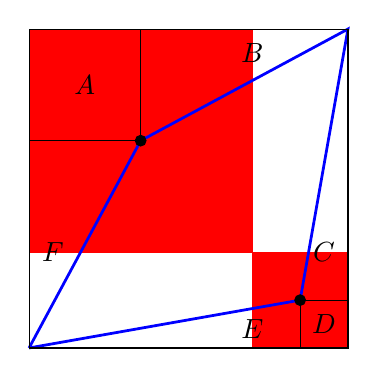
\begin{tikzpicture}
      \def\bss{9}
      \def\mpt{0.7}
      \coordinate (A) at (\mpt * \bss / 2, -\mpt * \bss / 2);
      \coordinate (B) at (\mpt * \bss /2 + \bss/2, -\mpt * \bss /2 - \bss/2);
      \filldraw[draw=black, color=red] (0, 0) rectangle (\mpt * \bss, -\mpt * \bss);
      \filldraw[draw=black, color=red] (\mpt * \bss, -\mpt * \bss) rectangle (\bss, -\bss);
      \draw[line width=1, color=blue] (0,-\bss) -- (A) -- (\bss, 0) -- (B) -- (0, -\bss);
      \draw[fill=black] (A) circle (0.15);
      \draw[fill=black] (B) circle (0.15);
      \draw (0,0) rectangle (\bss,-\bss);

      % Draw regions
      \draw (0,0) rectangle (A);
      \draw (B) rectangle (\bss, -\bss);

      % Region labels
      \draw (\mpt * \bss/4, -\mpt * \bss/4) node {$A$};
      \draw (\mpt * \bss, -0.075 * \bss) node {$B$};
      \draw (\bss - 0.075*\bss, -\mpt * \bss) node {$C$};
      \draw (0.75*\bss + \mpt * \bss / 4, -0.75*\bss - \mpt * \bss / 4) node {$D$};
      \draw (\mpt * \bss, -\bss + 0.06*\bss) node {$E$};
      \draw (0.075*\bss, -\mpt * \bss) node {$F$};
    \end{tikzpicture}
  \end{center}

  Now let $s$ be the side lengths of the black square and $s_u$ be the side lengths of the upper left red square, and define
  \gath{
    \a = \frac{s_u}{s}
  }
  as the side length of the upper left red square normalized to the large square side length.
  Clearly then $s_u = \a s$.
  These regions are reasoned to have the following areas:
  \ali{
    A_A &= \parens{\frac{\a s}{2}}^2 = \frac{\a^2 s^2}{4} \\
    A_B &= \frac{1}{2}\parens{\frac{\a s}{2}}\parens{s - \frac{\a s}{2}} = \frac{1}{2}\parens{\frac{\a s}{2}}\parens{\frac{(2-\a)s}{2}} = \frac{\a(2-\a)s^2}{8} \\
    A_C &= \frac{1}{2}\parens{\frac{(1-\a)s}{2}}\parens{s - \frac{(1-\a)s}{2}} = \frac{1}{2}\parens{\frac{(1-\a)s}{2}}\parens{\frac{(1+\a)s}{2}} = \frac{(1-\a^2)s^2}{8} \\
    A_D &= \parens{\frac{(1-\a)s}{2}}^2 = \frac{(1-\a)^2 s^2}{4} \\
    A_E &= A_C = \frac{(1-\a^2)s^2}{8} \\
    A_F &= A_B = \frac{\a(2-\a)s^2}{8} \,.
  }
  The area of the quadrilateral is then clearly
  \ali{
    A_Q &= s^2 - (A_A + A_B + A_C + A_D + A_E + A_F) = s^2 - A_A - 2A_B - 2A_C - A_D \non
    &= s^2 - \frac{\a^2 s^2}{4} - \frac{\a(2-\a)s^2}{4} - \frac{(1-\a^2)s^2}{4} - \frac{(1-\a)^2 s^2}{4} \non
    &= \frac{4s^2 - \a^2 s^2 - 2\a s^2 + \a^2 s^2 - s^2 + \a^2 s^2 - s^2 + 2\a s^2 - \a^2 s^2}{4} \non
    &= \frac{4s^2 - 2s^2}{4} = \frac{2s^2}{4} = \frac{s^2}{2} \,.
  }
  Thus the area of the black square is
  \gath{
    s^2 = 2A_Q = 2 \cdot 167 = 334 \,,
  }
  which of course is our answer.
}

\aproblem{13}{126}{\advent@xx@xiii}{
  Let $S(n, N)$ be the number of ways to split a sequence of the numbers 1 to $n$ into $N$ shorter sequences.
  First we note that it must be that $n \geq N$ as it is impossible to split $n$ numbers into more than $N = n$ shorter sequences.
  It is also clear that there is only one way to split $n$ numbers into a single sequence, namely the sequence itself.
  This of course translates to:
  \gath{
    \text{$S(n,1) = 1$ for all $n \geq 1$} \,. \label{eqn:pxiii:bc}
  }
  We also clearly have
  \gath{
    \text{$S(n, n) = 1$ for all $n \geq 1$} \label{eqn:pxiii:ext}
  }
  since there is only one way to split $n$ numbers into $n$ subsequences, namely that in which every subsequence contains only a single number.

  Now consider the general $S(n, N)$.
  If the first subsequence contains only the first number then there are $S(n-1, N-1)$ ways of splitting the remaining $n-1$ numbers into the remaining $N-1$ subsequences.
  If the first subsequence contains the first two numbers then there are $S(n-2, N-1)$ ways of splitting the remaining $n-2$ numbers into the remaining $N-1$ subsequences.
  In general, if the first subsequence contains $i$ numbers then there are $S(n-i, N-1)$ ways of splitting the remaining $n-i$ numbers into the remaining $N-1$ subsequences.
  This can continue until the number of remaining numbers equals the number of remaining subsequences, i.e. when the number of remaining numbers is $N-1$.
  Hence we have the following recursive relationship:
  \gath{
    S(n, N) = \sum_{i=N-1}^{n-1} S(i, N-1) = \sum_{i=N}^n S(i-1, N-1) \,. \label{eqn:pxiii:rec}
  }
  Here we note that
  \gath{
    S(n, n) = \sum_{i=n}^n S(i-1, n-1) = S(n-1, n - 1) = \cdots = S(1, 1) = 1
  }
  so that we have consistency and the condition \eqref{eqn:pxiii:ext} is not really explicitly necessary.

  The recursive function $S$ given by \eqref{eqn:pxiii:bc} and \eqref{eqn:pxiii:rec} was implemented in Python.
  When evaluated, the example results in the expected $S(5,3) = 6$, and the actual problem results in $S(10, 5) = 126$, which is of course our answer.
  We note that  we can find explicit formulas for $S(n,N)$ for specific $N$ iteratively.
  We know that we have $S(n,1) = 1$ in the $N=1$ case.
  For $N=2$ we have
  \gath{
    S(n,2) = \sum_{i=2}^n S(i-1, 1) = \sum_{i=2}^n 1 = n - 2 + 1 = n - 1 \,.
  }
  For $N=3$ we get
  \gath{
    S(n,3) = \sum_{i=3}^n S(i-1, 2) = \sum_{i=3}^n (i-1) - 1 = \sum_{i=3}^n (i-2) = \sum_{i=1}^{n-2} i = \frac{(n-2)(n-1)}{2} \,,
  }
  noting that again $S(5,3) = 6$ using this formula.
  However, beyond this point, things start to get very messy and that is why we just implemented the recursive formula in Python instead of determining an explicit formula for the $N = 5$ case.
}

\aproblem{14}{729}{\advent@xx@xiv}{
  This was solved with a brute force Python program that counts up all the numbers without duplicate digits.
}

\aproblem{15}{781}{\advent@xx@xv}{
  Logic was used to deduce the solution:
  \ali{
    A &= 8 & H &= 9 & S &= 7 & X &= 5 \non
    E &= 6 & M &= 1 & T &= 4 \non
    G &= 2 & R &= 3 & U &= 0
  }
  Thus our answer is $SAM = 781$.

  The full solution was verified with Python by checking the sums.
}

\aproblem{16}{333}{\advent@xx@xvi}{
  Logic was used to deduce this simple solution:

  \grid@advent@xx@xvi{3}{3}{3}{3}{3}{3}{3}{3}{3}

  This solution was verified with Python.
}

\aproblem{17}{189}{\advent@xx@xvii}{
  \boxans{\grid@advent@xx@xvii{6}{3}{7}{1}{2}{5}{4}{9}{8}}
}

\aproblem{18}{378}{\advent@xx@xviii}{
  In general, for $(x_1 + \cdots + x_n)^k$, each term in the expansion has $k$ of the original terms multiplied together.
  In the given example $n = k = 3$ so, for example, the $x^2 y$ term in the expansion still has $k = 3$ of the original terms, but $x$ is twice and $y$ once.
  Since order does not matter (for example of course the terms $x x y$, $xyx$, and $y x x$ all combine to make a single $x^2 y$ term), the number of terms in the expansion $N$ is the number of combinations with repetitions.
  This is known to be
  \gath{
    N(n, k) = \binom{n + k - 1}{k}    
  }
  in terms of the binomial coefficient.
  For the example, this results in $N(3, 3) = 10$ as expected.
  For the actual problem we get $N(3, 26) = 378$, which is of course our answer.
}

\aproblem{19}{512}{\advent@xx@xix}{
  Let $n$ denote the number of lines extending from one of the lower corners to divide up the opposite side into $n+1$ pieces.
  It is reasoned that this creates $n^2 + 2n = n(n+2)$ intersection points, including the intersections of the lines with the opposite sides of the original triangle.
  Each of these intersections form a triangle that includes the lower corner vertices.
  Hence, including the original triangle, the total number of triangles that involve both of the lower corner vertices is
  \gath{
    N_t(n) = n(n+2) + 1 \,.
  }
  All of the shapes formed by vertices in which none are one of the lower corner vertices are quadrilaterals.
  Thus every triangle \emph{must} involve one of the lower corner vertices.
  We have already counted the triangles involving \emph{both} of these vertices, so now we must count those involving only one of them (and two of the other vertices).
  There are $n+1$ lines extending from a corner vertex including one original side and not including the line to the other lower corner vertex.
  Each of these intersects lines from the other lower corner vertex (including the other original side) in $n+1$ places.
  We can choose any 2 of these intersection points to form a triangle having the other lower corner vertex as a vertex.
  Since this must be done for each of the $n+1$ lines and for each of the 2 lower corner vertices, it is reasoned that the number of these triangles is
  \gath{
    N_c(n) = 2(n+1)\binom{n+1}{2} \,.
  }
  Therefore the total number of triangles is
  \gath{
    N(n) = N_c(n) + N_t(n) = 2(n+1)\binom{n+1}{2} + n(n+2) + 1 \,.
  }
  As expected, this results in $N(2) = 27$ for the example, and it results in $N(7) = 512$ for the actual problem.
}

\aproblem{20}{234}{\advent@xx@xx}{
  This was solved with a brute force Python program.
  In particular, we have
  \ali{
    234 &= 14 + 15 + 16 + 17 + 18 + 19 + 20 + 21 + 22 + 23 + 24 + 25 \non
    234 &= 12 + 13 + 14 + 15 + 16 + 17 + 18 + 19 + 20 + 21 + 22 + 23 + 24 \,.
  }
}

\aproblem{21}{309}{\advent@xx@xxi}{
  This was solved using a brute force Python program.
  Try as I might, I could derive neither a general formula nor a recursive one.
  If $N(n)$ is the number of qualifying permutations for integers $\{1, \ldots, n\}$, then evidently the sequence $N(1), N(2), N(3), \ldots$ is \href{https://oeis.org/A000255}{OEIS A000255}.
  According to this there is no nice general formula but the sequence has the recursive relationship
  \ali{
    N(1) &= 1 \non
    N(2) &= 1 \non
    N(n) &= (n-1) N(n-1) + (n-2) N(n-2) \,,
  }
  which was verified with Python.
}

\aproblem{22}{984}{\advent@xx@xxii}{
  \boxans{\grid@advent@xx@xxii{9}{5}{4}{7}{2}{3}{8}{1}{6}}
}

\aproblem{23}{432}{\advent@xx@xxiii}{
  This was solved using a brute force Python program.
}

\aproblem{24}{812}{\advent@xx@xxiv}{
  Consider an $n \times n$ grid.
  There are two cases such that the required symmetry holds.
  The first is when both tokens are on the diagonal line of symmetry.
  Clearly there are $n$ such spaces and we must choose two on which to place the tokens.
  Thus the number of ways to do this is the same as choosing $2$ from $n$ combinations, i.e.
  \gath{
    \binom{n}{2}
  }
  in terms of a binomial coefficient.

  The second case is when neither token is on the diagonal and one of the tokens is to the left and below the diagonal, with the other token being on the corresponding space to the right and above the line of symmetry.
  It was reasoned that there are
  \gath{
    \sum_{i=1}^{n-1} i = \frac{n(n-1)}{2}
  }
  spaces on which to place the first token.
  Therefore the total number of ways to place the tokens and preserve the symmetry is
  \gath{
    N(n) = \binom{n}{2} + \frac{n(n-1)}{2} \,.
  }
  For the example, this formula yields $N(3) = 6$ as expected.
  For the actual problem, we then have $N(29) = 812$, which is of course our answer.
}

\end{document}
